\begin{itemize}
\item All the data can be tabularised as:
%
\begin{table}[!ht]
\centering
\resizebox{\columnwidth}{!}{\begin{tabular}{|c|c|c|c|} 
\hline
 & Fabricating&Finishing &Profit\\
\hline
\textbf{Model A} & 9  & 1 & 8000 \\ 
\hline
\textbf{Model B} & 12  & 3 & 12000 \\ 
\hline
\text{Max Hours} & $\leq180$&$\leq30$&\\
\hline
\end{tabular}}
\caption{Labour Hours and Profit for each piece}
\label{opt/2/35/tab:table1}
\end{table}
\item Let the number of pieces of model A manufactured be $x$ and
the number of pieces of model B manufactured be $y$ such that : 
\begin{align}
    x \geq 0 
    \\
    y \geq 0 
\end{align}
\item From the data given we have:
\begin{align}
    9x+12y &\leq 180 \\
    \implies 3x+4y&\leq60
\end{align}
and,
\begin{align}
    x+3y &\leq 30 
\end{align}

$\therefore$ The maximizing function is:
\begin{align}
        \max Z &= \myvec{8000& 12000}\vec{x}\\
        s.t. \quad 
        \myvec{3 & 4\\ 1 & 3 }\vec{x} &\preceq \myvec{60\\30} \\
        \vec{-x} &\preceq \vec{0}
\end{align}
\item The Lagrangian function can be given as:
\begin{equation}
\begin{aligned}
    &L(\vec{x},\boldsymbol{\lambda}) \\ &= \myvec{8000 & 12000}\vec{x}+\lcbrak{\sbrak{\myvec{3 & 4}\vec{x}-60}} \\ &+ \sbrak{\myvec{1 & 3}\vec{x}-30} \\ &+ \sbrak{\myvec{-1 & 0}\vec{x}} +\rcbrak{\sbrak{\myvec{0 & -1}\vec{x}}}\boldsymbol{\lambda}
\end{aligned}
\end{equation}
where,
\begin{align}
    \boldsymbol{\lambda} &= \myvec{\lambda_1 \\ \lambda_2 \\ \lambda_3 \\ \lambda_4}
\end{align}
\item Now, we have
\begin{align}
    \nabla L(\vec{x},\boldsymbol{\lambda}) &= \myvec{8000+ \myvec{3 & 1 & -1 & 0 }\boldsymbol{\lambda}\\ 12000+\myvec{4 & 3 &0 & -1}\boldsymbol{\lambda} \\ \myvec{3 & 4}\vec{x}-60 \\ \myvec{1 & 3}\vec{x}-30 \\ \myvec{-1 & 0}\vec{x} \\ \myvec{0 & -1}\vec{x}}
\end{align}
$\therefore$ The Lagrangian matrix is given by:-
\begin{align}
  \small{\myvec{0 & 0 & 3 & 1 & -1 & 0 \\ 0 & 0 & 4 & 3 &0 & -1 \\ 3 & 4 & 0 & 0 & 0 & 0 \\ 1 & 3 & 0 & 0 & 0 & 0 \\ -1 & 0 & 0 & 0 & 0 & 0 \\ 0 & -1 & 0 & 0 & 0 & 0 }\myvec{\vec{x} \\ \boldsymbol{\lambda} }}= \small{\myvec{-8000 \\ -12000 \\ 60 \\ 30 \\ 0 \\0 }}
\end{align}
\item Considering $\lambda_1,\lambda_2$ as only active multiplier,
\begin{align}
    \myvec{0 & 0 & 3 & 1  \\ 0 & 0 & 4 & 3 \\ 3 & 4 & 0 & 0 \\1 & 3 & 0 & 0}\myvec{\vec{x}\\ \boldsymbol{\lambda}} &= \myvec{-8000 \\ -12000 \\ 60 \\ 30}
\end{align}
\begin{align}
 \implies   \myvec{\vec{x} \\ \boldsymbol{\lambda}} &=  \myvec{0 & 0 & 3 & 1  \\ 0 & 0 & 4 & 3 \\ 3 & 4 & 0 & 0 \\1 & 3 & 0 & 0} ^{-1}\myvec{-8000 \\ -12000 \\ 60 \\ 30}
    \\
    \implies   \myvec{\vec{x} \\ \boldsymbol{\lambda}} &= \myvec{0 & 0 & \frac{3}{5} & \frac{-4}{5} \\ 0 & 0 & \frac{-1}{5} & \frac{3}{5} \\ \frac{3}{5} & \frac{-1}{5} & 0 & 0 \\ \frac{-4}{5} & \frac{3}{5} & 0 & 0}\myvec{-8000 \\ -12000 \\ 60 \\ 30}
    \\
    \implies \myvec{\vec{x} \\ \boldsymbol{\lambda}} &= \myvec{12 \\6 \\ -2400 \\ -800 }
\end{align}
$\because \boldsymbol{\lambda}=\myvec{-2400 \\ -800} \prec \vec{0}$
\\
\item The Optimal solution is given by:
\begin{align}
    \vec{x} &= \myvec{12\\6} \\
    Z &= \myvec{8000&12000}\vec{x} \\
   Z &= \myvec{8000&12000}\myvec{12 \\ 6} \\
    Z&= \text{Rs} 168000
\end{align}
\item So, to maximise profit
\\
 Pieces of model \textbf{A} manufactured is \boxed{x=12} and
 \\
  Pieces of model \textbf{B} manufactured is \boxed{y=6}.
\item The maximum profit per week is \boxed{Z=\text{Rs} 168000} .

\begin{figure}[!ht]
\centering
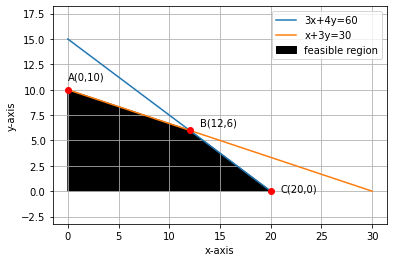
\includegraphics[width=\columnwidth]{solutions/su2021/2/35/Figure 10_1.png}
\caption{Graphical Representataion}
\end{figure}
\end{itemize}

